\documentclass{report}
\usepackage[utf8]{inputenc}
\usepackage[T1]{fontenc}
\usepackage{ifpdf}
\usepackage{cmap}
\usepackage{lmodern}
\usepackage{titlesec}
\usepackage{hyperref}
\usepackage{graphicx}
\usepackage{titling}
\usepackage{geometry}
\usepackage{titling}
\usepackage{tikz}
\usepackage{listings}
\usepackage{color}
\usepackage{minted}
\usepackage{caption}
\usetikzlibrary{trees}

\newcommand{\subtitle}[1]{%
  \posttitle{%
    \par\end{center}
    \begin{center}\large#1\end{center}
    \vskip0.5em}%
}

% Customize the caption label for listings
\renewcommand\listingscaption{Kód}

\geometry{
  top=4cm,    % Adjust the top margin as needed
  bottom=2cm, % Adjust the bottom margin as needed
  left=2.5cm, % Adjust the left margin as needed
  right=2.5cm % Adjust the right margin as needed
}

\titleformat{\chapter}
  {\Huge\bfseries}
  {\Huge\thechapter.}
  {0.5em}
  {}

\titlespacing*{\chapter}{0pt}{-2cm}{0.5cm}

\titleformat{\subsection}
  {\normalfont\large\bfseries}{\thesubsection}{0.7em}{}
\titlespacing*{\subsection}{0pt}{0.7em}{0.7em}

\hypersetup{
    colorlinks,
    citecolor=black,
    filecolor=black,
    linkcolor=black,
    urlcolor=black
}

\renewcommand\contentsname{Tartalomjegyzék}
\renewcommand\listoflistingscaption{Kódok}

\title{Email kliens fejlesztés - Projektmunka}
\subtitle{Fejlesztői dokumentáció}
\author{Tóth Balázs - MWZX0D}
\date{}

\pretitle{%
  \begin{center}
  \LARGE
  
\includegraphics[width=0.4\textwidth]{oe_logo.png}\\ % Adjust the width as needed
  \vspace{-7cm}
}

\begin{document}

\maketitle

\tableofcontents

\chapter{Projektek}
\graphicspath{ {./assets/} }

\chapter{DNS szerver}

\section{Indítás}
Ahhoz, hogy használni tudjuk az email klienst, kritikus fontosságú a DNS szervernek a futtatása. Természetesen arra vonatkozik ez a megkötés, ha lokálisan futtatjuk az email szervert!
\begin{itemize}
    \item \verb|docker-compose up -d|
\end{itemize}

\begin{flushleft}
    Parancs futtatása után látható, hogy sikeresen elindult a DNS szerver.
    \begin{center}
        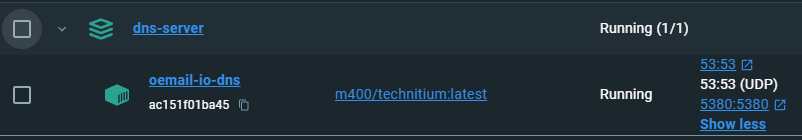
\includegraphics[width=0.9\textwidth]{docker-up-dns-server.png}
    \end{center}
\end{flushleft}

\section{Konfiguráció}
\begin{flushleft}
    Magát a konfigurációt webes környezetben hajthatjuk végre, amely látható is, hogy a \textbf{5380} porton fut. Cím, amelyen a konfigurációt elvégezhetjük:
    \begin{itemize}
        \item \verb|http://localhost:5380/|
    \end{itemize}
\end{flushleft}

\subsection{Zóna hozzáadása}
Megadott paraméterek:
\begin{itemize}
    \item Zóna neve: \verb|oemail.io|
    \item Típus: \verb|Primary Zone|
\end{itemize}

\subsection{Record hozzáadása}
\chapter{SMTP, IMAP szerver}

\section{hMailServer}
\begin{flushleft}
    Be kell kapcsolni az SMTP, IMAP protokollokat, ezután meg kell adni a megfelelő domain nevét: \verb|oemail.io|. Itt hozhatunk létre IMAP fiókokat is, amit az \verb|Accounts| menüpontban tehetünk meg.
    \begin{center}
        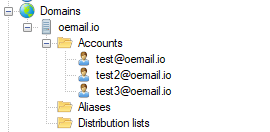
\includegraphics[width=0.5\textwidth]{hmailServer-accounts.png}
    \end{center}
\end{flushleft}

\section{Alapértelmezett mappák}
\begin{flushleft}
    Új fiók regisztrációja során az alábbi mappák kerülnek létrehozásra:
    \begin{itemize}
        \item \textbf{INBOX}: Bejövő emailek.
        \item \textbf{SENT}: Elküldött emailek.
        \item \textbf{TRASH}: Szemét, törölt emailek.
        \item \textbf{SPAM}: Gyanús emailek.
        \item \textbf{STARS}: Kedvenc emailek.
    \end{itemize}
\end{flushleft}
\chapter{Backend}

\section{Bejelentkezés}
\begin{itemize}
    \item Végpont - \textbf{/api/users/login}
    \begin{itemize}
        \item \textbf{POST} (JSON)
    \end{itemize}
    \item Előfeltétel(ek): \textbf{Nincs}
\end{itemize}
\begin{itemize}
    \item Bemeneti paraméter(ek):
    \begin{itemize}
        \item email - Típus: \textbf{email}
        \item password - Típus: \textbf{string}
    \end{itemize}
\end{itemize}
\begin{listing}[H]
    \begin{minted}[linenos, numbersep=-10pt]{json}
        {
            "email": "test2@oemail.io",
            "password": "test"
        }
    \end{minted}
    \caption{Példa adatok a bejelentkezéshez}
    \label{code:json_login}
\end{listing}

\section{Regisztráció}
\begin{itemize}
    \item Végpont - \textbf{/api/users/}
    \begin{itemize}
        \item \textbf{POST} (JSON)
    \end{itemize}
    \item Előfeltétel(ek): \textbf{Nincs}
\end{itemize}
\begin{itemize}
    \item Bemeneti paraméter(ek):
    \begin{itemize}
        \item user - Típus: \textbf{object}
    \end{itemize}
\end{itemize}
\begin{listing}[H]
    \begin{minted}[linenos, numbersep=-10pt]{json}
        {
            "user": {
                "email": "test2@oemail.io",
                "password": "test",
                "firstName": "Test2",
                "lastName": "Test2"
            }
        }
    \end{minted}
    \caption{Példa adatok a regisztrációhoz}
    \label{code:json_register}
\end{listing}

\newpage
\section{Adott email lekérése mappából}
\begin{itemize}
    \item Végpont - \textbf{/api/mail/getEmailByMailBox}
    \begin{itemize}
        \item \textbf{POST} (JSON)
    \end{itemize}
    \item Előfeltétel(ek): \textbf{Felhasználói bejelentkezés (token)}
\end{itemize}
\begin{itemize}
    \item Bemeneti paraméter(ek):
    \begin{itemize}
        \item mailBoxName - Típus: \textbf{string}
    \end{itemize}
\end{itemize}
\begin{listing}[H]
    \begin{minted}[linenos, numbersep=-10pt]{json}
        {
            "mailBoxName": "INBOX"
        }
    \end{minted}
    \caption{Példa adatok a legújabb email lekérésére adott mappából}
    \label{code:json_mailbox_one}
\end{listing}

\section{Összes email lekérése mappából}
\begin{itemize}
    \item Végpont - \textbf{/api/mail/getAllEmailByMailBox}
    \begin{itemize}
        \item \textbf{POST} (JSON)
    \end{itemize}
    \item Előfeltétel(ek): \textbf{Felhasználói bejelentkezés (token)}
\end{itemize}
\begin{itemize}
    \item Bemeneti paraméter(ek):
    \begin{itemize}
        \item mailBoxName - Típus: \textbf{string}
    \end{itemize}
\end{itemize}
\begin{listing}[H]
    \begin{minted}[linenos, numbersep=-10pt]{json}
        {
            "mailBoxName": "INBOX"
        }
    \end{minted}
    \caption{Példa adatok az összes email lekérésére adott mappából}
    \label{code:json_mailbox_all}
\end{listing}

\section{Email törlése mappából}
\begin{itemize}
    \item Végpont - \textbf{/api/mail/deleteMessage}
    \begin{itemize}
        \item \textbf{DELETE} (JSON)
    \end{itemize}
    \item Előfeltétel(ek): \textbf{Felhasználói bejelentkezés (token)}
\end{itemize}
\begin{itemize}
    \item Bemeneti paraméter(ek):
    \begin{itemize}
        \item mailBoxName - Típus: \textbf{string}
    \end{itemize}
\end{itemize}
\begin{listing}[H]
    \begin{minted}[linenos, numbersep=-10pt]{json}
        {
            "mailBoxName": "INBOX"
        }
    \end{minted}
    \caption{Példa adatok adott email törlésére mappából}
    \label{code:json_delete_email_mailbox}
\end{listing}

\section{Spam szűrés}
\begin{itemize}
    \item Végpont - \textbf{/api/mail/filterInboxFromSpam}
    \begin{itemize}
        \item \textbf{POST} (JSON)
    \end{itemize}
    \item Előfeltétel(ek): \textbf{Felhasználói bejelentkezés (token)}
\end{itemize}
\begin{itemize}
    \item Bemeneti paraméter(ek):
    \begin{itemize}
        \item mailBoxName - Típus: \textbf{string}
    \end{itemize}
\end{itemize}
\begin{listing}[H]
    \begin{minted}[linenos, numbersep=-10pt]{json}
        {
            "mailBoxName": "INBOX"
        }
    \end{minted}
    \caption{Példa adatok spam emailek szűrésére}
    \label{code:json_spam_email_mailbox}
\end{listing}

\section{Mappa létrehozása}
\begin{itemize}
    \item Végpont - \textbf{/api/mail/createMailBox}
    \begin{itemize}
        \item \textbf{POST} (JSON)
    \end{itemize}
    \item Előfeltétel(ek): \textbf{Felhasználói bejelentkezés (token)}
\end{itemize}
\begin{itemize}
    \item Bemeneti paraméter(ek):
    \begin{itemize}
        \item mailBoxName - Típus: \textbf{string}
    \end{itemize}
\end{itemize}
\begin{listing}[H]
    \begin{minted}[linenos, numbersep=-10pt]{json}
        {
            "mailBoxName": "INBOX"
        }
    \end{minted}
    \caption{Példa adatok mappa létrehozására}
    \label{code:json_new_email_mailbox}
\end{listing}

\section{Mappák lekérése}
\begin{itemize}
    \item Végpont - \textbf{/api/mail/listMailboxes}
    \begin{itemize}
        \item \textbf{GET}
    \end{itemize}
    \item Előfeltétel(ek): \textbf{Felhasználói bejelentkezés (token)}
\end{itemize}
\begin{itemize}
    \item Bemeneti paraméter(ek):
    \begin{itemize}
        \item Nincs
    \end{itemize}
\end{itemize}

\listoflistings

\end{document}